\documentclass[sigplan,screen]{acmart}

%%
%% \BibTeX command to typeset BibTeX logo in the docs
\AtBeginDocument{%
	\providecommand\BibTeX{{%
Bib\TeX}}}

\begin{document}

\title{GNU, Free software and Stallman's dedication}

\author{Stan Ioan-Victor, 832}
\email{ioan.victor.stan@stud.ubbcluj.ro}

\begin{teaserfigure}
	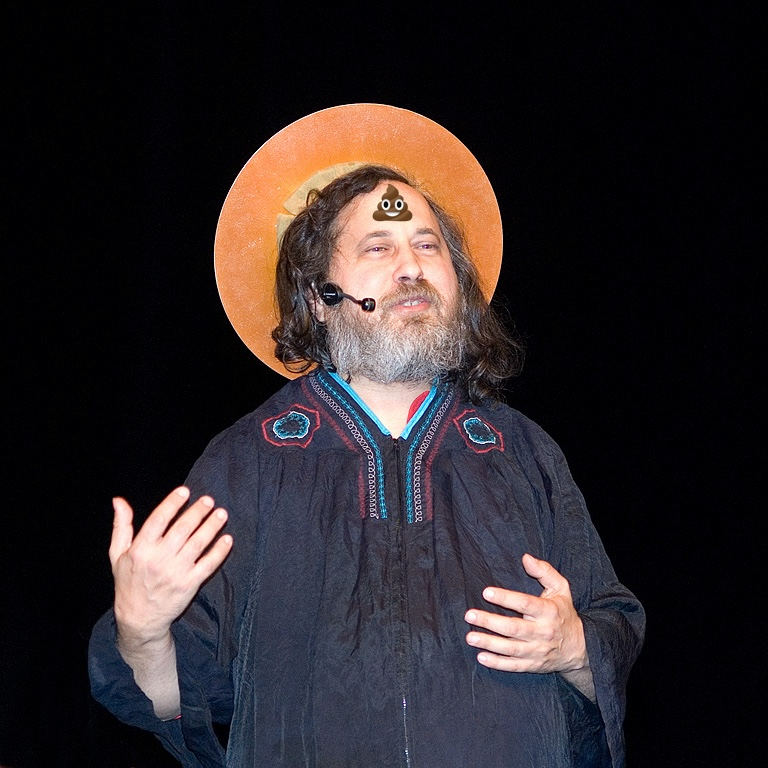
\includegraphics[width=200px]{pics/jesus-stallman.jpg}
	\centering
	\caption{RMS in his divine prime}
	\Description{Enjoying the baseball game from the third-base
	seats. Ichiro Suzuki preparing to bat.}
	\label{fig:teaser}
\end{teaserfigure}

%% This command processes the author and affiliation and title
%% information and builds the first part of the formatted document.
\maketitle

ACM's consolidated article template, introduced in 2017, provides a
consistent \LaTeX\ style for use across ACM publications, and
incorporates accessibility and metadata-extraction functionality
necessary for future Digital Library endeavors. Numerous ACM and
SIG-specific \LaTeX\ templates have been examined, and their unique
features incorporated into this single new template.

% ca na, sa ma lase sa compilez
\nocite{*}

\bibliographystyle{ACM-Reference-Format}
\bibliography{biblio}

%% If your work has an appendix, this is the place to put it.
% \appendix

\end{document}
\endinput
